\documentclass[11pt]{article}
\setlength{\parindent}{4em}
\title{Proposta de Projeto\\ EEL7801}
\author{Aluno: Carlos Freitas}
\date{24 de Agosto de 2023}
\renewcommand{\figurename}{Figura}

\usepackage{graphicx}
\usepackage{indentfirst}
\graphicspath{{images/}}

\begin{document}

\maketitle

\section*{Aspectos Gerais}

O projeto \textit{monitoring system} feito para a disciplina de
Projeto em Eletrônica I, de código EEL7801, tem como propósito monitorar
um ambiente específico, através de sensores, eletrônica embarcada e um servidor de modo
que seja possível registrar, organizar e processar os dados coletados para
cumprir determinados requisitos da finalidade do ambiente.

O design desse projeto seria composto por dois grandes blocos e pequenos
módulos que constituem esses blocos. Um diagrama que contém uma visão de alto
nível do projeto está na figura \ref{fig:diagram}.

\begin{figure}[h]
	\centering
	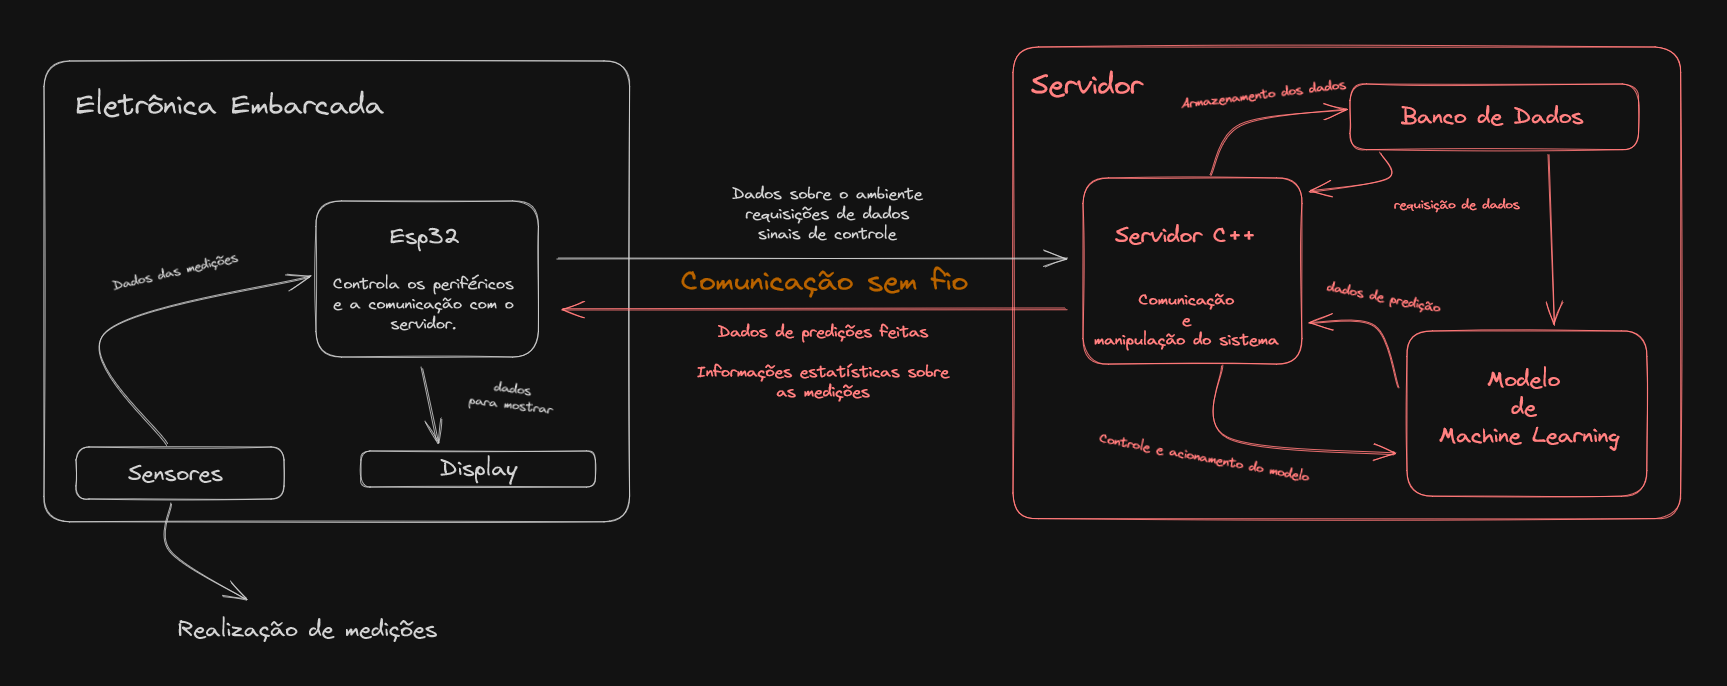
\includegraphics[width=0.85\textwidth,keepaspectratio]{diagramaprojetoI.png}
	\caption{Diagrama do projeto}
	\label{fig:diagram}
\end{figure}

\subsection*{Eletrônica embarcada}

O bloco de eletrônica embarcada, visto na figura \ref{fig:ee}, é responsável pela leitura das grandezas de interesse
a exemplo de temperatura, umidade, luminosidade, etc. Tal processo é controlado pelo
microcontrolador central um ESP32 e realizado pelos sensores, tendo realizadas as medidas
o esp fará um tratamento nesses dados de modo a ser mais conveniente enviar para o servidor,
além disso, atualizará o display periodicamente com dados atualizados. Há também a comunicação
com o servidor que será feita pelo microcontrolador, a qual servirá como ponte entre esses dois
blocos, tem como responsabilidade entregar as requisições do ESP32 para o server e controlar a
transferência de dados entre os dois processos.

\begin{figure}[h]
	\centering
	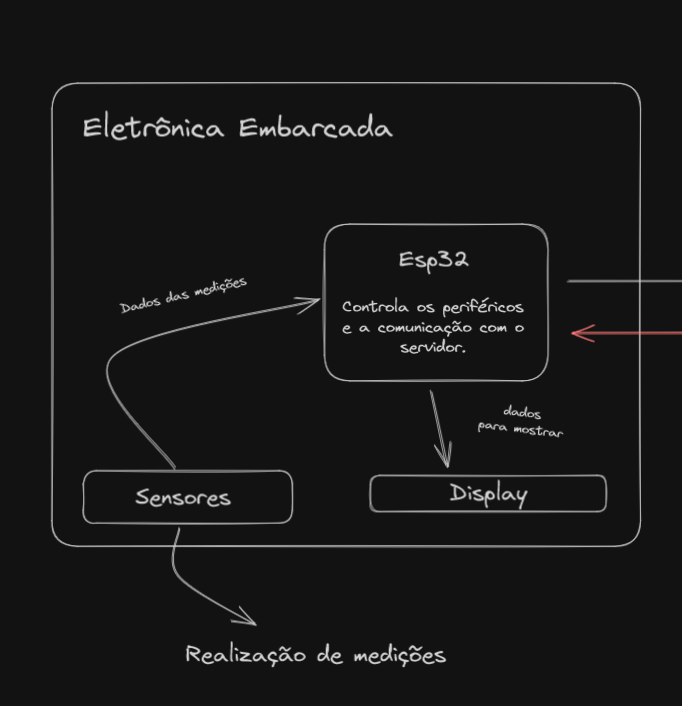
\includegraphics[width=0.85\textwidth,height=5cm,keepaspectratio]{ee.png}
	\caption{Diagrama do bloco embarcado}
	\label{fig:ee}
\end{figure}


\subsection*{Servidor}



\end{document}

